\documentclass[conference]{IEEEtran}
\usepackage[utf8]{inputenc}
\usepackage[T1]{fontenc}
\usepackage[spanish,es-tabla,es-nodecimaldot,es-noshorthands]{babel}
\usepackage{cite}
\usepackage{amsmath,amssymb,amsfonts}
\usepackage{graphicx}
\usepackage{booktabs}
\usepackage{array}
\usepackage{url}

\graphicspath{{figuras/}}

\begin{document}

\title{Simulación de un enlace de comunicaciones por luz visible en una galería de minería subterránea: confiabilidad y eficiencia bajo polvo, temperatura y maquinaria}

\author{\IEEEauthorblockN{Benjamín Morales}
\IEEEauthorblockA{\textit{Escuela de Informática y Telecomunicaciones} \\
\textit{Universidad Diego Portales}\\
Santiago, Chile \\
benjamin.morales3@mail.udp.cl}
\and
\IEEEauthorblockN{Philip Magna}
\IEEEauthorblockA{\textit{Escuela de Informática y Telecomunicaciones} \\
\textit{Universidad Diego Portales}\\
Santiago, Chile \\
philip.magna\_d@mail.udp.cl}
}

\maketitle

\begin{abstract}
Las comunicaciones por luz visible (VLC) son una alternativa a la radiofrecuencia en entornos industriales donde la interferencia electromagnética (EMI) degrada los enlaces convencionales. Este trabajo simula en MATLAB un enlace VLC en una galería de minería subterránea sometida a polvo, temperatura, maquinaria móvil e interferencia luminosa, y lo compara con Wi-Fi a 2.4~GHz y con un esquema híbrido VLC/Wi-Fi. El desempeño se evalúa mediante la tasa de error de bit (BER) sobre el tiempo disponible y el Goodput. El enlace óptico opera con un margen de 46.2~dB en aire limpio y soporta concentraciones muy superiores a los límites ocupacionales chilenos (DS~594) prácticamente sin errores, colapsando recién entre 1200 y 1500~mg/m$^{3}$. Frente a 40 obstrucciones por minuto, dos luminarias fijas elevan el Goodput de 6.56 a 8.27~Mb/s y reducen la BER de $6.0\times10^{-3}$ a $2.4\times10^{-3}$, superando a un selector práctico con información de canal ruidosa (7.05~Mb/s, BER $5.0\times10^{-2}$). A 5.4~m sin EMI, el Wi-Fi mantiene 9.41~Mb/s, pero cae a 1.03~Mb/s (80\,\% de indisponibilidad) con 50~dB de EMI, mientras que el esquema híbrido basado en dos luminarias fijas conserva 9.41~Mb/s y sostiene 5.85~Mb/s cuando ambos enlaces fallan simultáneamente.
\end{abstract}

\begin{IEEEkeywords}
comunicaciones por luz visible, minería subterránea, Industria 4.0, tasa de error de bit, Goodput.
\end{IEEEkeywords}

\section{Introducción}
La minería subterránea moderna demanda enlaces inalámbricos confiables para telemetría, monitoreo de seguridad y operación semiautónoma. En Chile, faenas de gran escala como la División El Teniente de Codelco operan en galerías profundas de geometría irregular, con polvo en suspensión, maquinaria pesada e intensa interferencia electromagnética (EMI) proveniente de subestaciones y equipos eléctricos~\cite{palacios2020}. En estas condiciones, los enlaces convencionales de radiofrecuencia (RF) sufren atenuación por obstáculos metálicos, dispersión multitrayecto e interferencia electromagnética.

Las comunicaciones por luz visible (VLC) aprovechan las luminarias LED existentes como transmisores en el espectro de 400 a 800~THz, aportando inmunidad total a la EMI sin requerir licencias de espectro~\cite{palacios2020,almadani2020}. Sin embargo, su desempeño depende fuertemente de la línea de vista (LOS) y de la extinción óptica producida por partículas en suspensión. Por ello, resulta relevante cuantificar en qué regímenes de operación conviene emplear VLC, Wi-Fi o una arquitectura híbrida.

Este trabajo simula un enlace VLC en una galería subterránea bajo polvo, temperatura elevada, maquinaria móvil e interferencia de focos, evaluando la confiabilidad (BER) y la eficiencia (Goodput) frente a Wi-Fi IEEE~802.11n (2.4~GHz) y a un esquema híbrido VLC/Wi-Fi. Se cuantifican además mitigaciones de diseño y operación orientadas a la implementación industrial.

\section{Trabajos relacionados}
El estudio de VLC en entornos industriales y mineros ha crecido sostenidamente en los últimos años. Revisiones como~\cite{almadani2020} sintetizan los desafíos de robustez y cobertura en plantas industriales, mientras que~\cite{berenguer2018} reporta mediciones experimentales de canal y transmisión MIMO óptica en un entorno fabril real.

Para minería subterránea específicamente, Palacios Játiva \emph{et al.}~\cite{palacios2020} propusieron un modelo de canal que integra inclinación de transmisores y receptores, paredes irregulares, sombra aleatoria por maquinaria mediante un proceso de Poisson y dispersión por polvo, aunque sin validación experimental directa. Posteriormente, el mismo grupo extendió el análisis incorporando distribuciones tridimensionales de polvo~\cite{palacios2022} y dependencia espectral de la atenuación con modulación CSK~\cite{becerra2023}. En paralelo, Javaid \emph{et al.}~\cite{javaid2021} analizaron el efecto del polvo de carbón sobre las componentes LOS y reflejada, Li \emph{et al.}~\cite{li2024} parametrizaron la extinción óptica por partículas mineras, e Iturralde \emph{et al.}~\cite{iturralde2024} propusieron un sistema híbrido VLC/RF para monitoreo de salud ocupacional en minas. A diferencia de trabajos centrados solo en la respuesta al impulso del canal, aquí se compara de forma integrada el desempeño a nivel de paquete (BER y Goodput) entre arquitecturas VLC, Wi-Fi y un esquema híbrido bajo condiciones combinadas.

\section{Escenario y modelo del sistema}

\subsection{Canal óptico y reflexiones}
El canal óptico sigue la formulación por trazado de rayos de~\cite{palacios2020}. Cada luminaria tiene patrón lambertiano de orden $m = -\ln 2 / \ln(\cos\Phi_{1/2})$, donde $\Phi_{1/2}$ es el semiángulo a media potencia. La ganancia en continua del enlace LOS a distancia $d$ es
\begin{equation}
H_{\mathrm{LOS}} =
\begin{cases}
\dfrac{(m+1)A_p}{2\pi d^{2}}\cos^{m}(\phi)\cos(\psi)\,g(\psi), & 0\le\psi\le\Psi_c,\\[2mm]
0, & \text{en otro caso,}
\end{cases}
\label{eq:hlos}
\end{equation}
con $A_p$ el área del fotodiodo, $\phi$ el ángulo de emisión, $\psi$ el de incidencia, $\Psi_c$ el campo de visión (FOV) y $g(\psi)=\eta^2/\sin^2\Psi_c$ la ganancia del concentrador óptico de índice $\eta$. La potencia recibida es $P_r = P_t\,H$ y la corriente fotogenerada es $R_{PD}P_r$.

Para las reflexiones difusas de primer orden en paredes, techo y piso (reflectividad $\rho_w$), las superficies se discretizan en elementos $\Delta A_w$~\cite{palacios2020,kahn1997}:
\begin{equation}
H_{\mathrm{NLOS}}=\sum_{w}\frac{(m+1)A_p\,\rho_w\,\Delta A_w}{2\pi^{2}d_{iw}^{2}d_{wj}^{2}}\cos^{m}(\phi_{iw})\cos(\alpha_w)\cos(\beta_w)\cos(\psi_{wj})\,g(\psi_{wj}),
\label{eq:nlos}
\end{equation}
donde $d_{iw}$ y $d_{wj}$ son las distancias luminaria-pared y pared-receptor, $\alpha_w$ y $\beta_w$ los ángulos respecto a la normal de la pared y $\tau=(d_{iw}+d_{wj})/c$ el retardo de cada trayecto. Agrupando en intervalos de 0.25~ns se obtiene la respuesta al impulso $h(t)$ y el retardo cuadrático medio $D_{\mathrm{RMS}}$, que acota la tasa sin interferencia intersímbolo a $R_b\le 1/(10\,D_{\mathrm{RMS}})$. Los parámetros ópticos se listan en la Tabla~\ref{tab:param}.

\begin{table}[!t]
\caption{Parámetros del sistema óptico~\cite{palacios2020}}
\label{tab:param}
\centering
\begin{tabular}{ll}
\toprule
\textbf{Parámetro} & \textbf{Valor}\\
\midrule
Potencia óptica emitida total, $P_t$ & 10 W \\
Semiángulo a media potencia, $\Phi_{1/2}$ & 60$^{\circ}$ ($m=1$) \\
Área activa del fotodiodo, $A_p$ & 1 cm$^{2}$ \\
Responsividad, $R_{PD}$ & 0.53 A/W \\
Semiángulo del campo de visión, $\Psi_c$ & 70$^{\circ}$ \\
Índice de refracción, $\eta$ & 1.5 \\
Ganancia del filtro óptico & 1 \\
\bottomrule
\end{tabular}
\end{table}

\subsection{Sombra, polvo, suciedad y temperatura}
Las obstrucciones (maquinaria y personal) llegan según un proceso de Poisson de intensidad $\epsilon$ y se modelan como cilindros verticales de diámetro $w\in U[0.5, 2.5]$~m y altura $h\in U[0.5, 3.5]$~m en posiciones uniformes del piso, con permanencia exponencial de media $T_d=30$~s. Estas dimensiones sustituyen al $U[0,2]$~m ilustrativo de~\cite{palacios2020}, que rara vez interceptaría un enlace hacia un casco a 1.8~m. La probabilidad estacionaria de enlace libre es
\begin{equation}
P=\exp\!\left[-\epsilon\,T_d\,E(p)\right],
\label{eq:sombra}
\end{equation}
donde $E(p)$ es la probabilidad de bloqueo por una obstrucción. El trayecto LOS usa la realización temporal exacta y las reflexiones usan la ponderación esperada $P_{iw}P_{wj}$~\cite{palacios2020}.

La atenuación por polvo en suspensión sigue la ley de Beer--Lambert $\exp(-\alpha L)$ sobre cada trayecto de longitud $L$, con coeficiente de extinción
\begin{equation}
\alpha=\frac{3\,Q_{\mathrm{ext}}\,C}{4\,\rho_p\,r},
\label{eq:polvo}
\end{equation}
donde $C$ es la concentración másica, $Q_{\mathrm{ext}}=2.2$ y $r=2~\mu$m~\cite{li2024}, y $\rho_p=1500$~kg/m$^3$, resultando $\alpha=5.5\times10^{-4}$~m$^{-1}$ por mg/m$^3$. La suciedad acumulada en los lentes se modela como una transmitancia neta $T_{\ell}$.

El efecto térmico sobre el LED reduce su eficiencia óptica $\eta(T_j)=\eta_0[1-k_T(T_j-25)]$ según la temperatura de juntura $T_j=T_a+R_{th}P_e(1-\eta(T_j))$, comparando un disipador estándar ($R_{th}=1.5$~K/W) y uno mejorado (0.8~K/W). El ruido del receptor sigue a~\cite{palacios2020,komine2004}:
\begin{align}
\sigma_0^{2}&=2q\,(I_{bg}+I_d)\,I_2B+\sigma_{th}^{2},\label{eq:s0}\\
\sigma_1^{2}&=\sigma_0^{2}+2q\,R_{PD}P_r\,B,\label{eq:s1}\\
\sigma_{th}^{2}&=\frac{8\pi\kappa T_K}{G}\,C_{pd}A_p\,I_2B^{2}+\frac{16\pi^{2}\kappa T_K\Gamma}{g_m}\,(C_{pd}A_p)^{2}I_3B^{3},\label{eq:th}
\end{align}
con $B=R_b$. La corriente oscura $I_d$ se duplica cada 10~K y la interferencia luminosa de focos vehiculares se representa como pulsos que elevan $I_{bg}$ (Tabla~\ref{tab:param2}). El receptor usa modulación todo-nada (OOK) con un \emph{umbral fijo} en la mitad de la corriente de señal sin bloqueo (no adaptativo ante caídas súbitas del LOS). El margen de enlace se define en escala de amplitud como $\mathrm{Margen~(dB)}=20\log_{10}(R_{PD}P_r/\sigma_1)$, de modo que 21.6~dB ($a=12$) equivale a $\mathrm{BER}\approx 10^{-9}$.

\begin{table}[!t]
\caption{Parámetros de temperatura, receptor y enlace}
\label{tab:param2}
\centering
\begin{tabular}{llc}
\toprule
\textbf{Parámetro} & \textbf{Valor} & \textbf{Origen}\\
\midrule
Eficiencia óptica a 25~$^{\circ}$C, $\eta_0$ & 0.30 & supuesto\\
Caída del flujo, $k_T$ & 0.4~\%/K & supuesto\\
Resistencia térmica, estándar / mejorado & 1.5 / 0.8~K/W & supuesto\\
Corriente oscura a 25~$^{\circ}$C, $I_d$ & 1~nA & supuesto\\
Corriente de fondo, $I_{bg}$ (y pulso focos) & 10~nA (50~$\mu$A) & \cite{palacios2020} / sup.\\
Ganancia $G$, $\Gamma$, $g_m$ del FET & 10, 1.5, 0.03~S & \cite{palacios2020}\\
Capacitancia $C_{pd}$ y factores $I_2, I_3$ & 112~pF/cm$^{2}$, 0.562, 0.0868 & \cite{palacios2020}\\
Tasa nominal, $R_b$ & 10~Mb/s & supuesto\\
Paquete y cabecera, $L$ y $n_p$ & 128 y 8 bits & supuesto\\
\bottomrule
\end{tabular}
\end{table}

\subsection{Geometría y punto de operación}
Como muestra la Fig.~\ref{fig:escenario}, se simula una galería de $26\times5\times4$~m con dos luminarias en el techo ($z=3.8$~m) sobre el eje central ($y=2.5$~m) en $x=8$~m y $x=18$~m, y un punto de acceso (AP) Wi-Fi ubicado junto a la luminaria~1. El receptor apunta hacia arriba a altura de casco ($z=1.8$~m) en el punto medio ($x=13$~m), a 5~m horizontales de cada luminaria. Con una diferencia de altura de 2~m, el ángulo de incidencia es $\psi=\arctan(5/2)\approx 68.2^{\circ}$, muy próximo al límite del campo de visión ($\Psi_c=70^{\circ}$), por lo que constituye el punto de menor margen con cobertura LOS simultánea. Las paredes tienen reflectividad $\rho=0.6$~\cite{palacios2020}, y el retardo cuadrático medio de la galería ($D_{\mathrm{RMS}}=0.075$~ns) permite tasas de hasta $\sim 1.3$~Gb/s, muy por encima de los 10~Mb/s simulados.

\begin{figure}[!t]
\centering
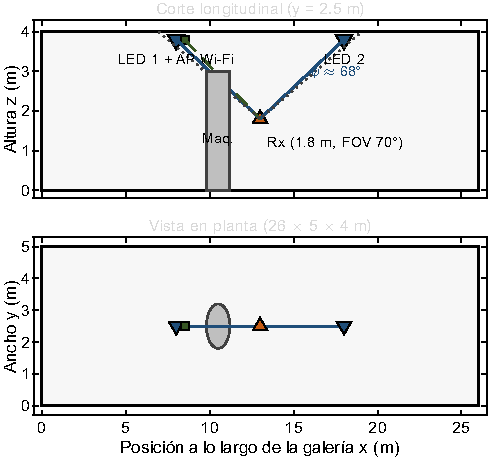
\includegraphics[width=\columnwidth]{fig_escenario}
\caption{Esquema de la galería minera simulada ($26\times5\times4$~m): corte longitudinal (arriba) y vista en planta (abajo), con las luminarias LED, el AP Wi-Fi, el receptor en el casco ($\psi\approx 68^{\circ}$) y una obstrucción cilíndrica.}
\label{fig:escenario}
\end{figure}

\section{Arquitecturas, métricas y validación}

\subsection{Arquitecturas y métricas de desempeño}
Se evalúan cuatro arquitecturas VLC manteniendo la misma potencia óptica total $P_t=10$~W: (1) \emph{1 LED} (solo luminaria~1), (2) \emph{2 LEDs fijos} (ambas luminarias emiten simultáneamente con potencia dividida 50/50), (3) \emph{selector ideal} (cota superior con conocimiento instantáneo perfecto del mejor enlace) y (4) \emph{selector práctico} (decide con información de canal cada 0.12~s, retardo de 0.06~s, error relativo del 8\,\%, histéresis del 5\,\%, corte de 25~ms por conmutación y 16~bits de pilotos adicionales).

El desempeño se mide con la BER calculada sobre el tiempo en que el enlace está disponible ($d_k\in[0,1]$) y el Goodput útil promedio $G$:
\begin{equation}
\mathrm{BER}=\frac{\sum_k d_k\,e_k/L}{\sum_k d_k},\qquad
G=\frac{R_b\,L}{L+n_p}\;\overline{d_k\,\mathbb{1}[e_k=0]},
\label{eq:metricas}
\end{equation}
donde $L=128$~bits, $n_p=8$~bits de cabecera base y $e_k$ son los bits erróneos del paquete $k$. De esta forma, tanto en VLC como en Wi-Fi la BER mide estrictamente errores de transmisión cuando hay enlace disponible, mientras que las caídas o conmutaciones penalizan el Goodput y la disponibilidad se reporta por separado.

\subsection{Enlace Wi-Fi y esquema híbrido}
El enlace de referencia Wi-Fi IEEE~802.11n (2.4~GHz, 20~MHz, 1 flujo espacial)~\cite{ieee80211n} transmite con $P_t=20$~dBm desde la luminaria~1 ($d=5.39$~m) y comparte exactamente las mismas obstrucciones. La pérdida sigue el modelo log-distancia con $n=2.2$ y sombreado lognormal ($\sigma=5$~dB), valores dentro del rango medido a 2.4~GHz en entornos industriales~\cite{tanghe2008}, sumando 15~dB cuando una máquina bloquea el trayecto. La EMI se modela como una elevación $\Delta_{\mathrm{EMI}}$ del piso de ruido térmico. El sistema selecciona el MCS más alto cuya sensibilidad cumple $P_r\ge S_{\mathrm{MCS}}+\Delta_{\mathrm{EMI}}$; si ninguno cumple, el enlace queda indisponible (Goodput nulo, sin asignar errores artificiales a la BER). La tasa útil es $\min(R_b,\,0.65\,R_{\mathrm{PHY}})$ y la BER se calcula para la modulación del MCS sin codificación.

El esquema híbrido opera por defecto sobre \emph{2~LEDs fijos} (la mejor arquitectura VLC práctica) y conmuta a Wi-Fi cuando la relación señal-ruido óptica cae por debajo de $Q=12$ y el enlace Wi-Fi está disponible, perdiendo un paquete en cada transición.

\subsection{Implementación, escenarios y validación}
La simulación de Monte Carlo se implementó íntegramente en MATLAB (R2026a, sin \emph{toolboxes} adicionales) con semilla fija y 40 réplicas independientes de 24~s (480 paquetes cada una); el código fuente y los datos generados están disponibles en \url{https://github.com/benjamin09111/vlc_2}. Para comparar escenarios de obstrucciones en igualdad de condiciones, se genera la tasa máxima (40 llegadas/min) y se conserva una fracción aleatoria en cada caso (\emph{thinning} de Poisson). Los intervalos de confianza del 95\,\% se calculan entre réplicas y todas las arquitecturas comparten las mismas secuencias de bits y ruido. La Tabla~\ref{tab:esc} resume los escenarios simulados.

\begin{table}[!t]
\caption{Escenarios simulados}
\label{tab:esc}
\centering
\begin{tabular}{lp{5.8cm}}
\toprule
\textbf{Grupo} & \textbf{Condición y valores}\\
\midrule
E0 & Referencia limpia (sin polvo, $T_\ell=1$, 25~$^{\circ}$C, sin obstr./EMI)\\
E1 & Polvo (mg/m$^{3}$): 25, 100, 300, 600, 1000, 1200, 1500, 2000\\
E2 & Transmitancia de los lentes, $T_\ell$: 0.8, 0.6, 0.4\\
E3 & Temperatura ambiente ($^{\circ}$C): 20, 30, 40, 50, 60 (dos disipadores)\\
E4 & Obstrucciones (llegadas/min): 5, 10, 20, 40\\
E5 & Interferencia luminosa de focos (8\,\% del tiempo)\\
E6 & Combinado: 1000~mg/m$^{3}$, $T_\ell=0.6$, 50~$^{\circ}$C, 10 obstr./min e interf.\\
E7 & Polvo 1200~mg/m$^{3}$ con 25, 40, 50 y 60~$^{\circ}$C y dos disipadores\\
E8 & EMI sobre Wi-Fi (dB sobre ruido térmico): 10, 20, 30, 40, 50\\
E9 & Fallas simultáneas: (a) 1500~mg/m$^{3}$, 10 obstr./min, EMI 40~dB; (b) E6 + EMI 40~dB\\
\bottomrule
\end{tabular}
\end{table}

El simulador se validó en tres frentes:
\begin{enumerate}
\item \emph{Canal de referencia~\cite{palacios2020}}: en el túnel de $6\times3\times5$~m, la Fig.~\ref{fig:cir} reproduce el arribo directo (9.16~ns) seguido de las reflexiones. Con la expresión impresa en~\cite{palacios2020} (que omite el factor $1/\pi$ de~\cite{kahn1997,komine2004}) la razón reflejado/directo es 10.1\,\% frente al 11.47\,\% reportado, mientras que la ecuación~\eqref{eq:nlos} completa da 3.2\,\% y es la usada en toda la galería. El retardo $D_{\mathrm{RMS}}=0.30$~ns cae dentro del amplio rango reportado ($9\times10^{-12}$ a $8.3\times10^{-9}$~s), aunque el pulso directo resulta 3.4 veces menor al publicado sin causa identificable en los parámetros impresos, por lo que esta validación es parcial.
\item \emph{BER Monte Carlo}: la Fig.~\ref{fig:ber} confirma que la simulación de $2\times10^{6}$ bits por punto coincide con la curva analítica $\tfrac{1}{2}\mathrm{erfc}(a/2\sqrt{2})$ dentro del IC~95\,\%.
\item \emph{Bloqueo de Poisson}: para $\epsilon=20$/min y $T_d=30$~s en 4000 réplicas, la fracción bloqueada simulada es $2.37\,\%\pm0.22\,\%$ frente a $2.12\,\%$ analítico de~\eqref{eq:sombra}; difieren levemente (alrededor de un error estándar) debido a la discretización temporal por paquetes y al tamaño de muestra.
\end{enumerate}

\begin{figure}[!t]
\centering
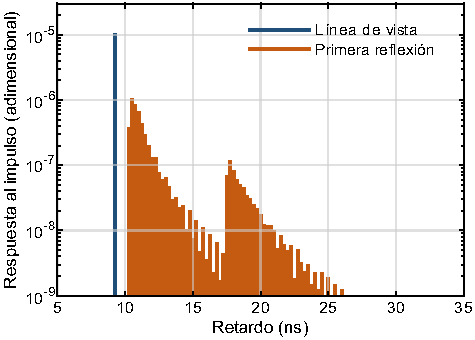
\includegraphics[width=\columnwidth]{fig_validacion_cir}
\caption{Respuesta al impulso del escenario de referencia de~\cite{palacios2020} calculada con la expresión impresa en dicho artículo ($\Delta t=0.25$~ns).}
\label{fig:cir}
\end{figure}

\begin{figure}[!t]
\centering
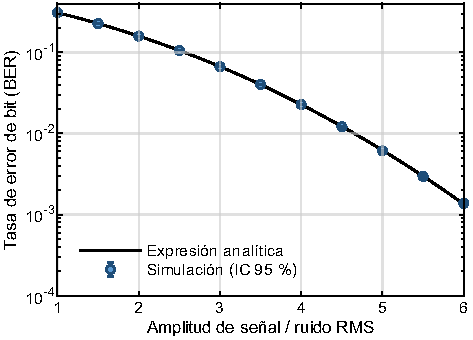
\includegraphics[width=\columnwidth]{fig_validacion_ber}
\caption{BER simulada ($2\times10^{6}$ bits/punto) frente a la expresión analítica OOK.}
\label{fig:ber}
\end{figure}

\section{Resultados}

\subsection{Cobertura y margen de enlace}
La Fig.~\ref{fig:cobertura} muestra el margen de enlace para dos luminarias fijas a 1.8~m de altura. En aire limpio, el margen en el punto de operación es de 46.2~dB y supera los 21.6~dB ($\mathrm{BER}\approx 10^{-9}$) en 20.5~m de los 26~m de la galería. Con 600~mg/m$^{3}$ de polvo el margen baja a 30.8~dB manteniendo los 20.5~m cubiertos, mientras que en la condición hostil (1000~mg/m$^{3}$, $T_\ell=0.6$, 50~$^{\circ}$C) cae a 14.6~dB y la zona cubierta se reduce a 15.0~m.

\begin{figure}[!t]
\centering
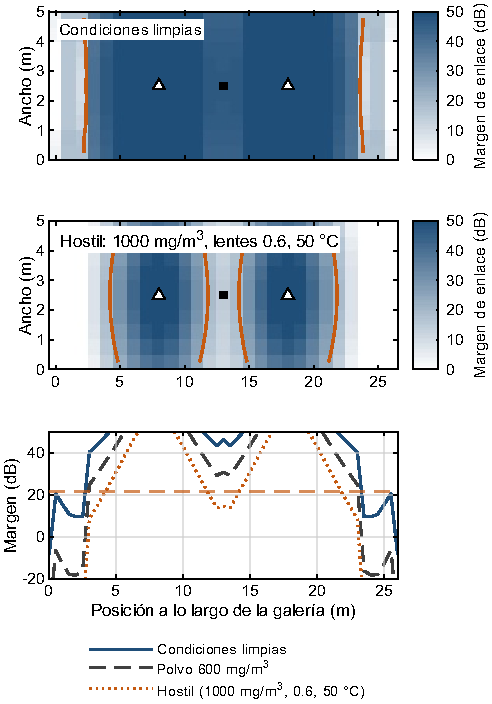
\includegraphics[width=\columnwidth]{fig_cobertura}
\caption{Margen de enlace de dos luminarias fijas a 1.8~m (arriba: limpio; centro: hostil; abajo: perfil longitudinal). La línea naranja marca 21.6~dB.}
\label{fig:cobertura}
\end{figure}

\subsection{Polvo, lentes y temperatura}
El polvo produce un colapso abrupto debido a la atenuación exponencial de Beer--Lambert (Fig.~\ref{fig:polvo}). Hasta 1000~mg/m$^{3}$, 1~LED y 2~LEDs fijos operan con BER nula y Goodput máximo de 9.41~Mb/s; a 1200~mg/m$^{3}$ la BER sube a $1.7\times10^{-3}$ (7.57~Mb/s), a 1500~mg/m$^{3}$ alcanza 0.11 con Goodput nulo, y a 2000~mg/m$^{3}$ llega a 0.39. En aire limpio, ni la suciedad de lentes ($T_\ell=0.4$), ni la temperatura (60~$^{\circ}$C), ni los focos vehiculares degradan el enlace gracias al amplio margen inicial. Sin embargo, cuando el polvo reduce el margen (1200~mg/m$^{3}$, Fig.~\ref{fig:temp}), subir a 60~$^{\circ}$C degrada el LED único a BER $1.1\times10^{-2}$ y 2.26~Mb/s con disipador estándar, mientras que el disipador mejorado duplica el Goodput a 4.52~Mb/s (BER $5.7\times10^{-3}$).

\begin{figure}[!t]
\centering
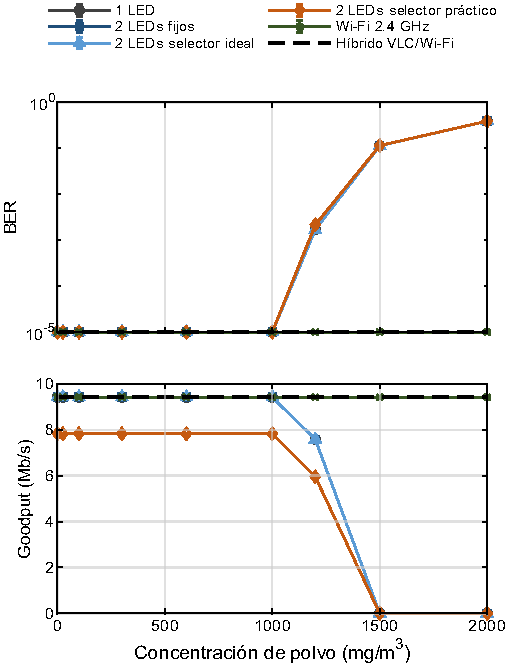
\includegraphics[width=\columnwidth]{fig_polvo}
\caption{BER y Goodput frente a la concentración de polvo, sin obstrucciones (IC~95\,\%).}
\label{fig:polvo}
\end{figure}

\begin{figure}[!t]
\centering
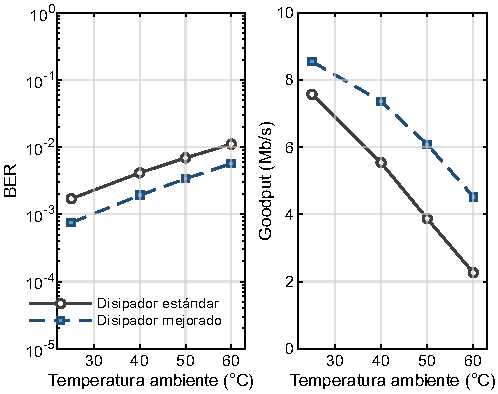
\includegraphics[width=\columnwidth]{fig_temperatura}
\caption{BER y Goodput del LED único frente a la temperatura con 1200~mg/m$^{3}$ de polvo para dos disipadores.}
\label{fig:temp}
\end{figure}

\subsection{Obstrucciones y arquitecturas ópticas}
Las obstrucciones son el factor dominante en aire limpio (Fig.~\ref{fig:obstr}). Con 40 llegadas/min, la luminaria~1 queda bloqueada el 33.8\,\% del tiempo: 1~LED cae a 6.56~Mb/s (BER $6.0\times10^{-3}$), mientras que 2~LEDs fijos logran 8.27~Mb/s (BER $2.4\times10^{-3}$), igualando prácticamente al selector ideal. El selector práctico, en cambio, rinde peor (7.05~Mb/s, BER $5.0\times10^{-2}$). Incluso sin obstrucciones (E0), el selector práctico pierde 1.59~Mb/s respecto a la suma fija (7.82 frente a 9.41~Mb/s): los 16~bits de pilotos reducen el techo en 10.5\,\%, y al estar el receptor equidistante de ambas luminarias ($x=13$~m), el error de estimación (8\,\%) supera la histéresis (5\,\%) y provoca 69 conmutaciones espurias por ciclo (7.15\,\% de interrupción). En el escenario combinado E6, 2~LEDs fijos obtiene 4.28~Mb/s (BER $3.5\times10^{-2}$) frente a 4.08~Mb/s (BER $2.0\times10^{-2}$) del selector práctico.

\begin{figure}[!t]
\centering
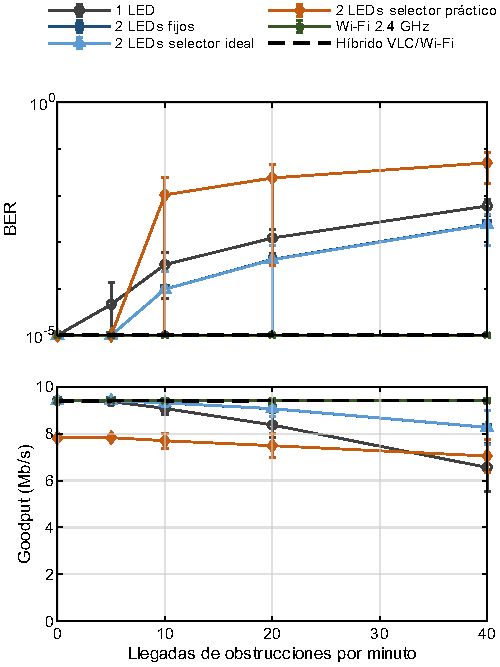
\includegraphics[width=\columnwidth]{fig_obstrucciones}
\caption{BER y Goodput frente a la intensidad de obstrucciones para las arquitecturas VLC, Wi-Fi e híbrido (IC~95\,\%).}
\label{fig:obstr}
\end{figure}

\subsection{Comparación con Wi-Fi y esquema híbrido}
La Tabla~\ref{tab:res} y la Fig.~\ref{fig:comp} comparan todas las arquitecturas. A 5.4~m sin EMI, el Wi-Fi mantiene 9.41~Mb/s y BER nula incluso con polvo denso o 40 obstrucciones/min. Al introducir EMI, su disponibilidad cae al 82.5\,\% con 40~dB (6.77~Mb/s) y al 20.0\,\% con 50~dB (1.03~Mb/s), aunque su BER condicional durante el tiempo disponible sigue siendo nula gracias al MCS robusto.

El esquema híbrido (basado en 2~LEDs fijos) elimina la penalización en aire limpio (9.41~Mb/s en E0) y mantiene 9.41~Mb/s tanto bajo 50~dB de EMI (operando en VLC) como bajo 1500~mg/m$^{3}$ de polvo o 40 obstrucciones/min (apoyándose en Wi-Fi). Cuando coinciden fallas severas (E9a: polvo 1500~mg/m$^{3}$, EMI 40~dB, 10 obstr./min), el VLC cae a 0 y el Wi-Fi opera el 72.1\,\% del tiempo con 5.85~Mb/s; el híbrido iguala ese Goodput (5.85~Mb/s) y recurre al VLC durante las caídas del Wi-Fi, resultando en una BER media de $5.9\times10^{-2}$. En E9b (E6 + EMI 40~dB), el híbrido supera a ambas tecnologías individuales alcanzando 6.66~Mb/s (BER $2.5\times10^{-2}$).

\begin{figure}[!t]
\centering
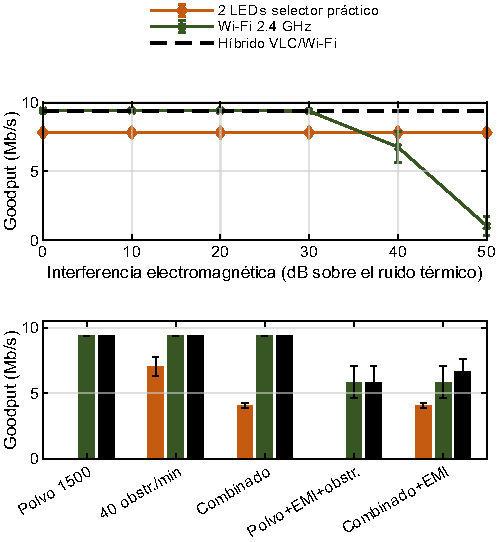
\includegraphics[width=\columnwidth]{fig_comparacion}
\caption{Arriba: Goodput frente a la EMI. Abajo: comparación en escenarios de falla severa y simultánea (EMI de 40~dB).}
\label{fig:comp}
\end{figure}

\begin{table*}[!t]
\caption{BER (sobre tiempo disponible) y Goodput $G$ (Mb/s) en escenarios representativos (promedio de 40 réplicas).}
\label{tab:res}
\centering
\footnotesize
\begin{tabular}{lccccccccccc}
\toprule
 & \multicolumn{2}{c}{1 LED} & \multicolumn{2}{c}{2 LEDs fijos} & \multicolumn{2}{c}{2 LEDs práctico} & \multicolumn{3}{c}{Wi-Fi 2.4 GHz} & \multicolumn{2}{c}{Híbrido (2 LEDs fijos)}\\
\cmidrule(lr){2-3}\cmidrule(lr){4-5}\cmidrule(lr){6-7}\cmidrule(lr){8-10}\cmidrule(lr){11-12}
\textbf{Escenario} & BER & $G$ & BER & $G$ & BER & $G$ & BER & Disp. & $G$ & BER & $G$\\
\midrule
Referencia (E0) & 0 & 9.41 & 0 & 9.41 & 0 & 7.82 & 0 & 100\,\% & 9.41 & 0 & 9.41 \\
Polvo 1000~mg/m$^3$ & 0 & 9.41 & 0 & 9.41 & 4.4$\times10^{-7}$ & 7.82 & 0 & 100\,\% & 9.41 & 0 & 9.41 \\
Polvo 1500~mg/m$^3$ & 1.1$\times10^{-1}$ & 0.00 & 1.1$\times10^{-1}$ & 0.00 & 1.2$\times10^{-1}$ & 0.00 & 0 & 100\,\% & 9.41 & 0 & 9.41 \\
10 obstr./min & 3.3$\times10^{-4}$ & 9.08 & 9.8$\times10^{-5}$ & 9.31 & 1.0$\times10^{-2}$ & 7.70 & 0 & 100\,\% & 9.41 & 0 & 9.41 \\
40 obstr./min & 6.0$\times10^{-3}$ & 6.56 & 2.4$\times10^{-3}$ & 8.27 & 5.0$\times10^{-2}$ & 7.05 & 0 & 100\,\% & 9.41 & 0 & 9.41 \\
Combinado (E6) & 5.6$\times10^{-2}$ & 4.82 & 3.5$\times10^{-2}$ & 4.28 & 2.0$\times10^{-2}$ & 4.08 & 0 & 100\,\% & 9.41 & 0 & 9.41 \\
EMI 40~dB & 0 & 9.41 & 0 & 9.41 & 0 & 7.82 & 0 & 82.5\,\% & 6.77 & 0 & 9.41 \\
Polvo 1500 + EMI 40 + 10 obstr. & 1.5$\times10^{-1}$ & 0.00 & 1.5$\times10^{-1}$ & 0.00 & 1.3$\times10^{-1}$ & 0.00 & 0 & 72.1\,\% & 5.85 & 5.9$\times10^{-2}$ & 5.85 \\
Combinado + EMI 40~dB & 5.6$\times10^{-2}$ & 4.82 & 3.5$\times10^{-2}$ & 4.28 & 2.0$\times10^{-2}$ & 4.08 & 0 & 72.1\,\% & 5.85 & 2.5$\times10^{-2}$ & 6.66 \\
\bottomrule
\end{tabular}
\end{table*}

\subsection{Mitigaciones y densidad de luminarias}
La Fig.~\ref{fig:mit} muestra que la alta BER del selector práctico con 40 obstr./min se debe al uso de una estimación ruidosa para fijar el umbral: calcular el umbral con pilotos del propio paquete baja su BER de $5.0\times10^{-2}$ a $2.4\times10^{-3}$ (7.14~Mb/s en E4 y 4.40~Mb/s en E6), igualando la confiabilidad de 2~LEDs fijos pero con menor Goodput en obstrucciones (7.14 frente a 8.27~Mb/s). Con 1200~mg/m$^{3}$ de polvo, limpiar los lentes recupera el Goodput del LED único desde 0 ($T_\ell=0.4$) a 2.77~Mb/s ($T_\ell=0.8$) y 7.57~Mb/s ($T_\ell=1.0$). Reducir la tasa a 5~Mb/s recupera el enlace a 1500~mg/m$^{3}$ (2.79~Mb/s, BER $4.1\times10^{-3}$), aunque no basta a 2000~mg/m$^{3}$. En el híbrido, cualquier umbral $Q\ge 8$ (incluido $Q=12$) logra 9.41~Mb/s en E4 y E6.

En el análisis estático de densidad (Fig.~\ref{fig:dens}), pasar de 2 a 3 luminarias (una cada 8.7~m, misma potencia total) eleva la cobertura con 10 obstr./min de 82.3\,\% a 97.8\,\% (y de 69.5\,\% a 86.3\,\% con 40/min), eliminando las zonas sin LOS en los extremos. Agregar una cuarta luminaria apenas mejora un punto porcentual en aire limpio, pero con 600~mg/m$^{3}$ de polvo y 40 obstr./min cada luminaria adicional sigue aportando (60.2\,\%, 75.1\,\%, 79.8\,\% y 82.8\,\% para $N=2,3,4,6$).

\begin{figure}[!t]
\centering
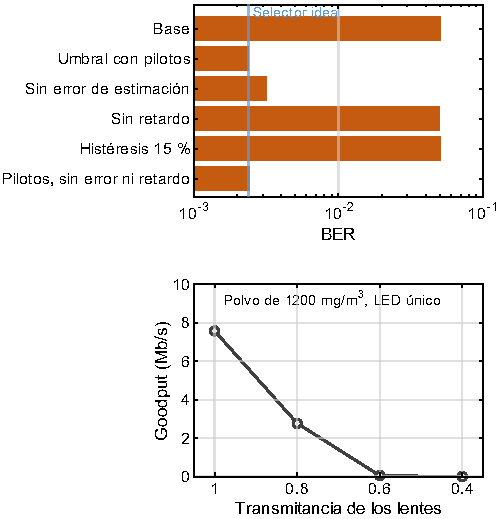
\includegraphics[width=\columnwidth]{fig_mitigaciones}
\caption{Arriba: BER del selector práctico con 40 obstr./min según mitigación. Abajo: efecto de la transmitancia de lentes con 1200~mg/m$^{3}$.}
\label{fig:mit}
\end{figure}

\begin{figure}[!t]
\centering
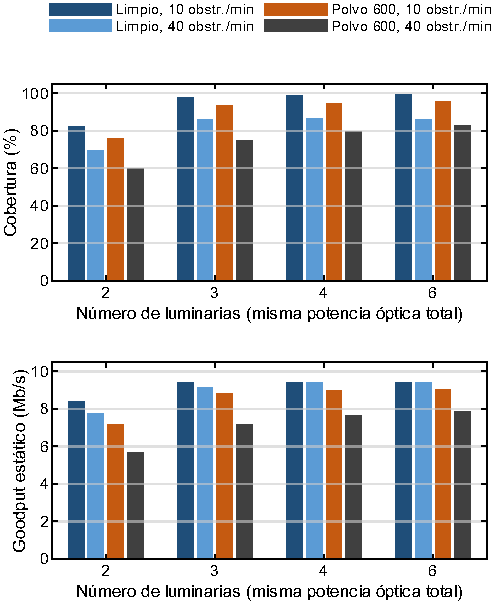
\includegraphics[width=\columnwidth]{fig_densidad}
\caption{Cobertura ($\ge 21.6$~dB) y Goodput estático frente al número de luminarias (400 instantáneas, 51 posiciones).}
\label{fig:dens}
\end{figure}

\section{Desafíos, limitaciones y contexto normativo}
Los resultados evidencian tres compromisos clave. Primero, la dependencia del LOS hace que, aun con 46.2~dB de margen, un vehículo bloquee el trayecto directo y haga caer la señal bajo el umbral fijo del receptor. Segundo, la atenuación exponencial por polvo provoca un colapso abrupto entre 1200 y 1500~mg/m$^{3}$. En la normativa chilena (Decreto Supremo N.°~594~\cite{ds594}), los límites permisibles ponderados para polvo respirable de sílice (cuarzo: 0.08~mg/m$^{3}$) y polvo total no especificado (8.0~mg/m$^{3}$) son órdenes de magnitud menores; por ende, bajo operación regular el VLC es totalmente robusto frente al polvo, y el rango de colapso simulado representa únicamente eventos extremos transitorios (como tronaduras o nubes densas locales tras carguío). Tercero, a 5.4~m sin EMI el Wi-Fi supera al VLC, por lo que el despliegue de VLC o híbrido se justifica específicamente en zonas con alta EMI o distancias mayores donde la RF se degrade.

Como limitaciones del estudio, la validación frente a~\cite{palacios2020} es parcial (el pulso directo difiere en un factor 3.4), las reflexiones consideran solo primer orden sobre paredes planas y el polvo se modela como medio atenuador homogéneo sin dispersión hacia el receptor~\cite{palacios2022}. Asimismo, los parámetros térmicos, dimensiones de maquinaria, ruido de focos y parámetros RF ($n=2.2$, $\sigma=5$~dB a una sola distancia fija) son supuestos de ingeniería sin medición en faena, y el análisis de densidad de luminarias es estático; por ello, las cifras representan tendencias relativas y requieren validación experimental en galería antes de fijar criterios de diseño definitivo.

\section{Recomendaciones y conclusiones}
Para una implementación industrial práctica se desprenden cuatro lineamientos:
\begin{enumerate}
\item \emph{Redundancia simple por suma fija}: iluminar cada tramo con al menos dos luminarias transmitiendo en simultáneo (espaciado $\le 8.7$~m, tres luminarias en 26~m) iguala la confiabilidad del selector ideal sin complejidad de conmutación ni pérdidas por estimación ruidosa.
\item \emph{Mantenimiento guiado por polvo y tasa adaptativa}: dado que el enlace colapsa abruptamente al superar 1200~mg/m$^{3}$ y es muy sensible a la suciedad de lentes en ese régimen, la limpieza óptica debe activarse por concentración de polvo (eventos de carguío/tronadura) y complementarse con reducción de tasa (5~Mb/s) y mejor disipación térmica en zonas calurosas.
\item \emph{Arquitectura híbrida coherente}: en sectores expuestos a EMI ($\ge 40$~dB) o distancias mayores, conviene emplear un esquema híbrido basado en \emph{2~LEDs fijos} con respaldo Wi-Fi, evitando selectores ópticos inestables.
\item \emph{Verificación de cobertura}: el espaciamiento entre luminarias debe diseñarse considerando el mapa de margen en condición hostil (Fig.~\ref{fig:cobertura}) y no solo en aire limpio.
\end{enumerate}

En conclusión, la simulación integrada en MATLAB demuestra que ninguna tecnología resiste por sí sola todos los modos de falla de una galería subterránea: el VLC con redundancia de luminarias garantiza inmunidad a la EMI y operación libre de errores bajo los límites legales de polvo, mientras que el Wi-Fi aporta resiliencia frente a obstrucciones y nubes extremas de polvo. Su combinación mediante un esquema híbrido simple maximiza la disponibilidad y el Goodput del enlace.

\section*{Declaración de uso de inteligencia artificial}
Se utilizaron herramientas de inteligencia artificial generativa únicamente como apoyo para mejorar la redacción, claridad y estilo del manuscrito. La formulación del modelo, la implementación y validación en MATLAB, la ejecución de las simulaciones y el análisis de los resultados son responsabilidad exclusiva de los autores.

\begin{thebibliography}{00}
\bibitem{palacios2020} P. Palacios Játiva \emph{et al.}, ``A VLC channel model for underground mining environments with scattering and shadowing,'' \emph{IEEE Access}, vol. 8, pp. 185445--185464, 2020, doi: 10.1109/ACCESS.2020.3030615.
\bibitem{almadani2020} Y. Almadani \emph{et al.}, ``Visible light communications for industrial applications---Challenges and potentials,'' \emph{Electronics}, vol. 9, n.º 12, art. 2157, 2020, doi: 10.3390/electronics9122157.
\bibitem{berenguer2018} P. W. Berenguer \emph{et al.}, ``Optical wireless MIMO experiments in an industrial environment,'' \emph{IEEE J. Sel. Areas Commun.}, vol. 36, n.º 1, pp. 185--193, 2018, doi: 10.1109/JSAC.2017.2774618.
\bibitem{palacios2022} P. Palacios Játiva \emph{et al.}, ``An enhanced VLC channel model for underground mining environments considering a 3D dust particle distribution model,'' \emph{Sensors}, vol. 22, n.º 7, art. 2483, 2022, doi: 10.3390/s22072483.
\bibitem{becerra2023} R. Becerra \emph{et al.}, ``A wavelength-dependent visible light communication channel model for underground environments and its performance using a color-shift keying modulation scheme,'' \emph{Electronics}, vol. 12, n.º 3, art. 577, 2023, doi: 10.3390/electronics12030577.
\bibitem{javaid2021} F. Javaid, A. Wang, M. U. Sana, A. Husain e I. Ashraf, ``Characteristic study of visible light communication and influence of coal dust particles in underground coal mines,'' \emph{Electronics}, vol. 10, n.º 8, art. 883, 2021, doi: 10.3390/electronics10080883.
\bibitem{li2024} C. Li \emph{et al.}, ``Study on VLC channel model in underground mining scenarios with extinction effect and shadowing effect,'' \emph{Appl. Opt.}, vol. 63, n.º 14, 2024, doi: 10.1364/AO.520073.
\bibitem{iturralde2024} D. Iturralde \emph{et al.}, ``A new Internet of Things hybrid VLC/RF system for m-Health in an underground mining industry,'' \emph{Sensors}, vol. 24, n.º 1, art. 31, 2024, doi: 10.3390/s24010031.
\bibitem{kahn1997} J. M. Kahn y J. R. Barry, ``Wireless infrared communications,'' \emph{Proc. IEEE}, vol. 85, n.º 2, pp. 265--298, feb. 1997.
\bibitem{komine2004} T. Komine y M. Nakagawa, ``Fundamental analysis for visible-light communication system using LED lights,'' \emph{IEEE Trans. Consum. Electron.}, vol. 50, n.º 1, pp. 100--107, feb. 2004.
\bibitem{ieee80211n} IEEE Std 802.11n-2009, ``Amendment 5: Enhancements for higher throughput,'' IEEE, 2009.
\bibitem{tanghe2008} E. Tanghe \emph{et al.}, ``The industrial indoor channel: Large-scale and temporal fading at 900, 2400, and 5200 MHz,'' \emph{IEEE Trans. Wireless Commun.}, vol. 7, n.º 7, pp. 2740--2751, 2008, doi: 10.1109/TWC.2008.070143.
\bibitem{ds594} Ministerio de Salud de Chile, ``Decreto Supremo N.° 594: Reglamento sobre condiciones sanitarias y ambientales básicas en los lugares de trabajo,'' 1999 (act. vigente).
\end{thebibliography}

\end{document}
